
\documentclass{beamer}
\usepackage[utf8]{inputenc}
\usepackage{url}
\usepackage{algorithm}
\usepackage{algpseudocode}
\usepackage{lmodern}
\usepackage{natbib}
\usepackage{tikz}
\usepackage{physics}
\usepackage{graphicx}
\usepackage{listings}

\graphicspath{ {./images/} }
\usepackage{booktabs}
\usepackage{tikz}
\usetikzlibrary{circuits.logic.US, positioning}

\usetikzlibrary{arrows.meta}

\usetikzlibrary{mindmap, trees, shadows, shapes, calc, fadings, positioning, decorations.pathreplacing, intersections, shapes, arrows}



\lstdefinestyle{python}{
  basicstyle=\ttfamily\scriptsize,
  keywordstyle=\color{blue},
  commentstyle=\color{gray},
  stringstyle=\color{red},
  showstringspaces=false,
  tabsize=2,
  breaklines=true
}


\usetheme{default}
\usepackage{graphics}

\usepackage{color}
\definecolor{new_turquoise}{RGB}{40,151,158}
\setbeamercolor{title}{fg=new_turquoise}




\makeatletter
\setbeamertemplate{frametitle}{
    \ifbeamercolorempty[bg]{frametitle}{}{\nointerlineskip}%
    \@tempdima=\textwidth%
    \advance\@tempdima by\beamer@leftmargin%
    \advance\@tempdima by\beamer@rightmargin%
    \vspace*{0.8cm} 

    \begin{beamercolorbox}[sep=0.3cm,center,wd=\the\@tempdima]{frametitle}
        \usebeamerfont{frametitle}%
        \vbox{}\vskip-1ex%
        \if@tempswa\else\csname beamer@ftecenter\endcsname\fi%
        \strut\insertframetitle\strut\par%
        {%
            \ifx\insertframesubtitle\@empty%
            \else%
            {\usebeamerfont{framesubtitle}\usebeamercolor[fg]{framesubtitle}\insertframesubtitle\strut\par}%
            \fi
        }%
        \vskip-1ex%
        \if@tempswa\else\vskip-.3cm\fi
    \end{beamercolorbox}%
}
\makeatother

\setbeamercolor{frametitle}{fg=new_turquoise}
\setbeamertemplate{itemize item}{\color{new_turquoise}$\blacksquare$}
\setbeamertemplate{itemize subitem}{\color{new_turquoise}$\blacksquare$}


\setbeamertemplate{enumerate item}{\color{new_turquoise}\insertenumlabel}
\setbeamertemplate{enumerate subitem}{\color{new_turquoise}\insertsubenumlabel}

\setbeamertemplate{caption}{\raggedright\insertcaption\par}

\setbeamercolor{section in toc}{fg=new_turquoise}
\setbeamercolor{subsection in toc}{fg=new_turquoise}
\setbeamercolor{subsubsection in toc}{fg=new_turquoise}



\setbeamercolor{block title}{fg=white, bg=new_turquoise}
\setbeamercolor{block body}{fg=black, bg=new_turquoise!10}

\setbeamercolor{block title}{fg=white, bg=new_turquoise}
\setbeamercolor{block body}{fg=black, bg=new_turquoise!10}


\usebackgroundtemplate{
    \includegraphics[width=\paperwidth,height=\paperheight]{figs/slide-title.jpg}
} 

\title{\fontsize{49}{7.2}{\bf Fundamental Algorithmic Techniques I}}
\date{\color{new_turquoise}\today}

\begin{document}
\frame{\titlepage}


\usebackgroundtemplate{
    \includegraphics[width=\paperwidth,height=\paperheight]{figs/slide-pages}
} 


\setbeamertemplate{subsection in toc}{
  \color{new_turquoise}$\blacksquare$\color{black}~~\inserttocsubsection
}


\begin{frame}{Outline}
    \tableofcontents
\end{frame}





\section{Finite Functions \& Circuits}


\begin{frame}{Finite functions \& Computing}
  \textcolor{new_turquoise}{Finite functions}:
  \[
   \mathcal{F}:\,  \{0, 1\}^n \longrightarrow \{0, 1\}^m
  \] \\
  \bigskip
  Computational Space: $\{0, 1\}^n \rightarrow \{0, 1\}$ with $2^{2^n}$ possibilities! \\
  
  \medskip 
  Examples: Hashing, encryption, boolean circuits
  \bigskip
  \bigskip
  \bigskip
  \bigskip
  \bigskip

  \textcolor{new_turquoise}{Computation}:\\
  \begin{itemize}
    \item \textcolor{new_turquoise}{Circuit}: $\mathcal{C}$ {\it computes} $\mathcal{F}$ if $\forall x \in \{0, 1\}^n, \mathcal{C}(x) = \mathcal{F}(x)$
    \item \textcolor{new_turquoise}{Program}: $\mathcal{P}$ {\it computes} $\mathcal{F}$ if $\forall x \in \{0, 1\}^n, \mathcal{P}(x) = \mathcal{F}(x)$ 
  \end{itemize}
\end{frame}


\begin{frame}{Basic Circuits: AND, OR, NOT}
\centering
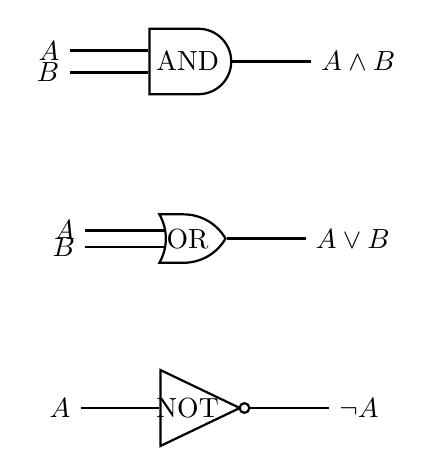
\begin{tikzpicture}[circuit logic US, thick]
  \node[and gate, inputs=nn] (and1) {AND};
  \node[left=of and1.input 1] (a1) {$A$};
  \node[left=of and1.input 2] (b1) {$B$};
  \node[right=of and1.output] (c1) {$A \land B$};
  \draw (a1) -- (and1.input 1);
  \draw (b1) -- (and1.input 2);
  \draw (and1.output) -- (c1);
  
  \node[or gate, inputs=nn, below=1.5cm of and1] (or1) {OR};
  \node[left=of or1.input 1] (a2) {$A$};
  \node[left=of or1.input 2] (b2) {$B$};
  \node[right=of or1.output] (c2) {$A \lor B$};
  \draw (a2) -- (or1.input 1);
  \draw (b2) -- (or1.input 2);
  \draw (or1.output) -- (c2);
  
  \node[not gate, below=1.5cm of or1] (not1) {NOT};
  \node[left=of not1.input] (a3) {$A$};
  \node[right=of not1.output] (c3) {$\lnot A$};
  \draw (a3) -- (not1.input);
  \draw (not1.output) -- (c3);
\end{tikzpicture}
\end{frame}


\begin{frame}{Basic Circuits: NAND}
\centering
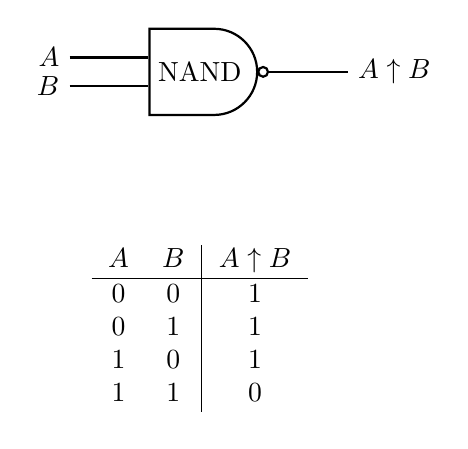
\begin{tikzpicture}[circuit logic US, thick]
  \node[nand gate, inputs=nn] (nand1) {NAND};
  \node[left=of nand1.input 1] (a1) {$A$};
  \node[left=of nand1.input 2] (b1) {$B$};
  \node[right=of nand1.output] (c1) {$A \uparrow B$};
  \draw (a1) -- (nand1.input 1);
  \draw (b1) -- (nand1.input 2);
  \draw (nand1.output) -- (c1);
  
  \node[below=1.5cm of nand1] (table) {
    \begin{tabular}{c c|c}
      $A$ & $B$ & $A \uparrow B$ \\
      \hline
      0 & 0 & 1 \\
      0 & 1 & 1 \\
      1 & 0 & 1 \\
      1 & 1 & 0 \\
    \end{tabular}
  };
\end{tikzpicture}\\
\medskip
{\bf Combinations of NAND gates generate OR/AND/NOT}\\
{\it functionally complete} Operator
\end{frame}


\section{Equivalence Relations}



\begin{frame}{Equivalence: Circuits $\Leftrightarrow$ Straight-Line Programs}
  \begin{columns}[T]
    \column{0.5\textwidth}
    \centering
    \includegraphics[width=\linewidth]{Algos_figs/circuitasacycligraph.png} \\
    \small  A Boolean circuit is a labeled acyclic graph (DAG)

    \column{0.5\textwidth}
    \centering
    \includegraphics[width=\linewidth]{Algos_figs/equivGraphStraightlineProgram.png} \\
    \small Boolean functions have
    straight-line program equivalents \footnote{\tiny AON is And, Or, Not CIRC for circuit...}
  \end{columns}

  \vspace{0.4cm}
  \centering
  \textbf{Equivalence $\Leftrightarrow$}: simply via topological sorting
\end{frame}





\begin{frame}[fragile]{MAJ and XOR: Code vs Circuits}
  \begin{columns}[T]
    \column{0.5\textwidth}
    \textbf{MAJ Implementation:}
    \begin{lstlisting}[style=python]
def MAJ(X[0],X[1],X[2]):
    firstpair = AND(X[0],X[1])
    secondpair = AND(X[1],X[2])
    thirdpair = AND(X[0],X[2])
    temp = OR(secondpair,thirdpair)
    return OR(firstpair,temp)
    \end{lstlisting}

    \vspace{0.5cm}
    \textbf{XOR Implementation:}
    \begin{lstlisting}[style=python]
def XOR(a,b):
    w1 = AND(a,b)
    w2 = NOT(w1)
    w3 = OR(a,b)
    return AND(w2,w3)
    \end{lstlisting}

    \column{0.5\textwidth}
    \centering
    \textbf{MAJ Circuit} \\
    \vspace{0.1cm}
    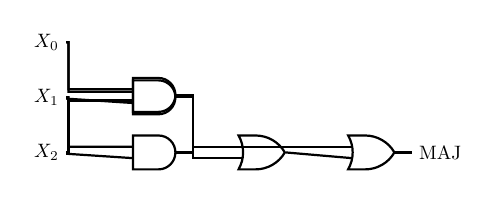
\begin{tikzpicture}[circuit logic US, thick, scale=0.7, transform shape]
  \node (x0) at (0,2) {$X_0$};
  \node (x1) at (0,1) {$X_1$};
  \node (x2) at (0,0) {$X_2$};
  
  \node[and gate, inputs=nn, right=1.2cm of x1] (and1) {};
  \node[and gate, inputs=nn, right=1.2cm of x2] (and2) {};
  \node[and gate, inputs=nn, above=0.4cm of and2] (and3) {};
  
  \draw (x0) -- ++(0.4,0) |- (and1.input 1);
  \draw (x1) -- (and1.input 2);
  \draw (x1) -- ++(0.4,0) |- (and2.input 1);
  \draw (x2) -- (and2.input 2);
  \draw (x0) -- ++(0.4,0) |- (and3.input 1);
  \draw (x2) -- ++(0.4,0) |- (and3.input 2);
  
  \node[or gate, inputs=nn, right=1.2cm of and2] (or1) {};
  \node[or gate, inputs=nn, right=1.2cm of or1] (or2) {};
  
  \draw (and2.output) -- ++(0.3,0) |- (or1.input 1);
  \draw (and3.output) -- ++(0.3,0) |- (or1.input 2);
  \draw (and1.output) -- ++(0.3,0) |- (or2.input 1);
  \draw (or1.output) -- (or2.input 2);
  
  \node[right=0.3cm of or2] (out) {MAJ};
  \draw (or2.output) -- (out);
\end{tikzpicture}

\vspace{0.8cm}
\textbf{XOR Circuit} \\
\vspace{0.1cm}
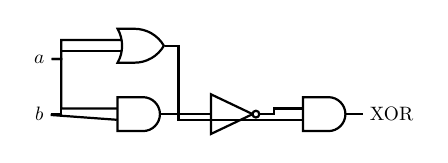
\begin{tikzpicture}[circuit logic US, thick, scale=0.7, transform shape]
  \node (a) at (0,1) {$a$};
  \node (b) at (0,0) {$b$};
  
  \node[and gate, inputs=nn, right=1.2cm of b] (and1) {};
  \draw (a) -- ++(0.4,0) |- (and1.input 1);
  \draw (b) -- (and1.input 2);
  
  \node[not gate, right=0.9cm of and1] (not1) {};
  \draw (and1.output) -- (not1.input);
  
  \node[or gate, inputs=nn, above=0.6cm of and1] (or1) {};
  \draw (a) -- ++(0.4,0) |- (or1.input 1);
  \draw (b) -- ++(0.4,0) |- (or1.input 2);
  
  \node[and gate, inputs=nn, right=0.9cm of not1] (and2) {};
  \draw (not1.output) -- ++(0.25,0) |- (and2.input 1);
  \draw (or1.output) -- ++(0.25,0) |- (and2.input 2);
  
  \node[right=0.3cm of and2] (out) {XOR};
  \draw (and2.output) -- (out);
    \end{tikzpicture}
  \end{columns}
\end{frame}





\begin{frame}{Computation of Finite Functions}
\begin{theorem}
\footnotesize
Every function $f: \{0, 1\}^n \to \{0, 1\}^m$ can be computed by a Boolean circuit of size at most
\[
\mathcal{O}\left(\frac{m \cdot 2^n}{n}\right)
\]
using AND, OR, and NOT gates.
\end{theorem}

\vspace{0.2cm}
\begin{corollary}
\footnotesize

Since AON computable by NAND, the same function can be computed by a NAND-only circuit of comparable size.
\end{corollary}

\vspace{0.2cm}
\begin{corollary}
Any such function can be represented by a single-line program of length $\mathcal{O}(m \cdot 2^n)$ using truth-table enumeration (e.g., via conditional expressions or lookup tables).
\end{corollary}
\end{frame}


\begin{frame}{Equivalence: Circuits $\leftrightarrows$ Code $\leftrightarrows$ Binary Data}
  \begin{block}{Circuit Encoding Theorem}
    Any Boolean circuit with $n$ gates can be represented using \\
    $\mathcal{O}(n \log n)$ bits.
  \end{block}

  \vspace{0.4cm}
  \textbf{Why?} Each gate requires:
  \begin{itemize}
    \item $\mathcal{O}(\log n)$ bits to specify its \textbf{type} (AND/OR/NOT)
    \item $\mathcal{O}(\log n)$ bits to specify its \textbf{input wires} (from $\leq n$ wires)
  \end{itemize}

  \vspace{0.2cm}
  \textbf{Total}: $n \cdot \mathcal{O}(\log n) = \mathcal{O}(n \log n)$ bits
\end{frame}







\section{Towards Realistic Computing?}


\begin{frame}{Larger Code $\Leftrightarrow$ Larger Circuits!}
  \begin{columns}[T]
    \column{0.5\textwidth}
    \centering
    \includegraphics[width=0.8\linewidth]{Algos_figs/z0nxq4cbski71.jpg} \\
    \vspace{0.2cm}
    \includegraphics[width=0.8\linewidth]{Algos_figs/chipcomputer.jpeg} \\
    \vspace{0.1cm}
    \small Circuits become larger and powerful via composition

    \column{0.5\textwidth}
    \centering
    \includegraphics[width=\linewidth]{Algos_figs/SyntacticSugar.png}
    Syntaxic Sugar \& Composition to compute any function!
  \end{columns}
\end{frame}


\section{Other Players and Limitations}


\begin{frame}{Universal Circuits \& Programs}
    Universal circuits/Programs are able to evaluage other circuits (Compiler, Interpreters, Browser, JIT, Emulators, Universal Turing Machines, ...).
    
\includegraphics[width=0.8\linewidth]{Algos_figs/UniversalPrograms.png}
    
\end{frame}



\begin{frame}{Landscape}
  Finite functions have a whole range of circuits/code lengths, with many rapidly 
  requiring exponentially long circuits as complexity grows:\\
  \begin{center}    
    \includegraphics[width=0.6\linewidth]{Algos_figs/finiteOverview.png}
  \end{center}
  {\bf So we need more powerful models for real-world computing!}
\end{frame}








\section{Infinite Functions and Turing Machines}



\begin{frame}{Introducing Infinite Functions}
\textcolor{new_turquoise}{Infinite Functions}: 
  \[
   \mathcal{F}:\,  \{0, 1\}^* \longrightarrow \{0, 1\}^*,
  \]
  with $\{0, 1\}^*$ standing for arbitrary length bit-strings.
  \bigskip

Examples: real-world computations \\
\begin{itemize}
    \item Compilers (arbitrary program size)
    \item Network protocols (variable packet lengths)
    \item Compression algorithms (any input size)
    \item AI models (token sequences of varying length)
\end{itemize} 

\bigskip
\textcolor{new_turquoise}{New notions to explore:}
\begin{itemize}
    \item Finite automaton and their limitations
    \item Turing machines alternative and its advantages
    \item Computability and Turing equivalence
\end{itemize}

\end{frame}



\begin{frame}{From Finite to Infinite Functions}
  \footnotesize
\textcolor{new_turquoise}{Finite functions} (circuits):
\begin{itemize}
    \item Handle fixed-size inputs: $\{0,1\}^n \to \{0,1\}^m$
    \item Can compute any function, but may require exponentially many gates
    \item \textbf{Limitation}: Cannot handle unbounded input sizes
\end{itemize}

\vspace{0.4cm}
\textcolor{new_turquoise}{Infinite functions} (unbounded computation):
\begin{itemize}
    \item Handle variable-length inputs: $\{0,1\}^* \to \{0,1\}^*$
    \item Real-world applications need this capability
    \item \textbf{Challenge}: Need computational models with unbounded memory
\end{itemize}

\vspace{0.4cm}
\textcolor{new_turquoise}{Path forward:}
\begin{itemize}
    \item Start with \textbf{Finite Automata} (limited memory)
    \item Progress to \textbf{Turing Machines} (unbounded memory)
    \item Understand \textbf{computability} and what can/cannot be computed
\end{itemize}

\end{frame}


\begin{frame}{Deterministic Finite Automaton (DFA)}
  \footnotesize 
  
  \begin{block}{DFA Robot}
    \begin{itemize}
      \item Reads input symbols (e.g., 0s and 1s) \textbf{one at a time}
      \item Decides to \textbf{accept} or \textbf{reject} the whole string
      \item Has \textbf{no memory} beyond its current state
    \end{itemize}
  \end{block}
  
  \vspace{0.3cm}
  \textbf{Key components:}
  \begin{itemize}
    \item \textbf{States}: Finite set (e.g., ``waiting'', ``success'', ``error'')
    \item \textbf{Start state}: Where the robot begins
    \item \textbf{Accept states}: Success states (double circle in diagrams)
    \item \textbf{Rules}: ``If in state $A$ and read symbol $x$, go to state $B$''
  \end{itemize}
  
  \vspace{0.4cm}
  Efficient for Regular Expressions!\\
  {\bf BUT} Infinitely many functions non computable
  by DFA in $\{0, 1\}^* \longrightarrow \{0, 1\}$
\end{frame}
  


\begin{frame}{Turing Machines: Why and How?}

\vspace{0.3cm}
\textcolor{new_turquoise}{Finite circuits (combinational logic):}\\
Can compute any \textbf{fixed-size} function $f: \{0,1\}^n \to \{0,1\}^m$.\\
But  \textbf{exponentially many gates} for general functions ($\sim 2^n/n$).\\
\textbf{Cannot handle unbounded inputs} (e.g. arbitrary lengths)

\vspace{0.2cm}
\textcolor{new_turquoise}{Deterministic Finite Automata (DFAs):}\\
Handle \textbf{unbounded input streams} with constant memory
but are \textbf{too weak} for basic tasks.


\vspace{0.5cm}
\textbf{Turing Machines add two critical capabilities:}
\begin{itemize}
    \item \textbf{Dynamic computation}: Modify state based on tape contents
    \item \textbf{Unbounded memory}: Read/write tape of infinite length
    \item \textbf{Turing Church Thesis}: Can compute any function

\end{itemize}
\end{frame}



\begin{frame}{Computability \& Turing Equivalence}
  \footnotesize
  \textbf{Computable Functions:} \\
  Let $F: \{0,1\}^* \to \{0,1\}$. A Turing machine $M$ \textit{computes} $F$ if:
  \[
  \forall x \in \{0,1\}^*, \quad M(x) \text{ halts with output } F(x)
  \]

  \vspace{0.4cm}
  \textcolor{new_turquoise}{\textbf{Turing Completeness}} \\
  A computational model is \textbf{Turing complete} if it can compute 
  \textit{exactly the same functions} as  (or simulate) a Turing machine.

  \vspace{0.5cm}
  \textbf{Equivalent Models:} (equivalent means Turing $\leftrightarrows$ Model simulable)
  \begin{itemize}
    \item \textbf{NAND-TM}: NAND-based Turing-complete language
    \item \textbf{RAM machines}: Standard computer architecture (registers, memory)
    \item \textbf{$\lambda$-calculus}: Function-based computation (Church's model)
    \item \textbf{Cellular automata}: e.g., Conway's Game of Life (2D grid rules)
  \end{itemize}
\end{frame}



\begin{frame}{Turing equivalent Models}
  Church-Turing Conjecture:   {\it Any function on natural numbers can be calculated by an effective method $\Leftrightarrow$ can be computed by a Turing machine.}
  
  \includegraphics[width=\linewidth]{Algos_figs/equicalentToTuring.png}
\end{frame}




\begin{frame}{Turing Machine: Simple Definition}
  \scriptsize
  A \textbf{Turing Machine} is a theoretical computer with:
  \begin{columns}[T]
    \column{0.6\textwidth}
    \textbf{3 Key Components:}
    \begin{enumerate}
      \item \textbf{Infinite tape} \\
      (like a never-ending strip of paper)
      \item \textbf{Read/write head} \\
      (can read, write, and move left/right)
      \item \textbf{State register} \\
      (remembers current "mode" of operation)
    \end{enumerate}

    \textbf{How it works:}
    \begin{itemize}
      \item Starts in \textbf{initial state}
      \item At each step:
        \begin{enumerate}
          \item Read symbol under head
          \item Write new symbol (or keep same)
          \item Move head \textbf{L} or \textbf{R}
          \item Switch to new state
        \end{enumerate}
      \item Halts when reaching \textbf{accept} or \textbf{reject} state
    \end{itemize}
    \column{0.4\textwidth}
    \centering
    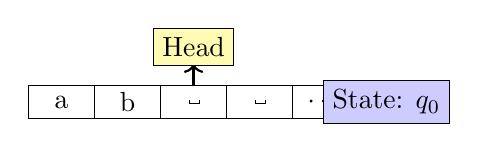
\begin{tikzpicture}[scale=0.7]
      \foreach \i in {0,...,4}
        \draw (1.2*\i,0) rectangle (1.2*\i+1.2,0.6);
      \node at (0.6,0.3) {a};
      \node at (1.8,0.3) {b};
      \node at (3.0,0.3) {\textvisiblespace};
      \node at (4.2,0.3) {\textvisiblespace};
      \node at (5.4,0.3) {$\cdots$};
      
      \draw[thick, ->] (3.0,0.6) -- (3.0,1.0);
      \node[draw, rectangle, fill=yellow!30] at (3.0,1.3) {Head};
      
      \node[draw, rectangle, fill=blue!20] at (6.5,0.3) {State: $q_0$};
    \end{tikzpicture}
    \vspace{0.7cm}

    \includegraphics[width=\linewidth]{Algos_figs/alan-turing-and-turing-machine.jpg}
  \end{columns}

  \vspace{0.2cm}
  \textbf{Key idea:} Can compute \textit{anything computable}!
\end{frame}




\begin{frame}{Summary}

  \begin{columns}[onlytextwidth]
  \column{0.5\textwidth}
  \textbf{Models of Computation}
  \begin{itemize}
      \item \textbf{Circuits} → finite, fixed-size programs (exponential lengths...)
      \item \textbf{Automata} → handle infinite inputs/outputs, but limited to regular/simple problems
      \item \textbf{Turing Machine}\\
      \begin{itemize}
      \item One per problem
          \item Infinite, writable tape
          \item Finite set of inner states
          \item Transition function/table 
      \end{itemize}
  
      \item \textbf{Universal Turing Machine}\\
      Programmable computer!
  \end{itemize}
  
  
  
  \column{0.5\textwidth}
  \small
  \textbf{Turing-Complete Systems}
  
  \begin{itemize}
      \item NAND-TM language
      \item RAM model (e.g., Python, C)
      \item Lambda calculus (e.g., Lisp, OCaml, Clojure)
      \item Cellular automata (e.g., Conway’s Game of Life)
  \end{itemize}
  
  \vfill
  \begin{center}
  \textcolor{new_turquoise}{\bf Church–Turing Thesis:} \\ 
  \textit{A function on natural numbers is effectively computable} \\
  $\Leftrightarrow$ \\
  \textit{It is computable by a Turing machine.}
  \end{center}
  \end{columns}
  
  \end{frame}




  \section{Computability and Computational Classes}




\begin{frame}{Incomputability by Turing Machine}
  One can prove that {\bf infinitely many} functions:
  $$\mathcal{F}: \{0,1\}^* \to \{0,1\}$$ are \textcolor{new_turquoise}{\bf uncomputable} by a Turing Machine.

  \bigskip
  Well-known examples:
  \begin{itemize}
    \item {\bf Halting Problem}: \\
    $\mathrm{Halt}(M, x) = 
    \begin{cases}
        1 & \text{if Turing machine } M \text{ halts on input } x, \\
        0 & \text{otherwise}.
    \end{cases}$ \\
    This function is uncomputable. \\

    \item {\bf Busy Beaver}: \\
    For an $n$-state Turing machine $M_n$, find the maximum number of steps $M_n$ can run before halting (over all inputs and all such machines). Grows faster than any computable function!
  \end{itemize}
  In Summary: 
  Two kind of uncomputable functions: by logical construction or growing too fast!
\end{frame}


\begin{frame}{Computational Complexity Classes — The Big Picture}
  \centering
  \scriptsize
  \textbf{Decision problems} (answer: Yes/No)
  
  \vspace{0.3cm}
  \begin{tabular}{@{}p{2.2cm}p{4.5cm}p{3.5cm}@{}}
    \toprule
    \textbf{Class}       & \textbf{Meaning}                              & \textbf{Example}             \\ 
    \midrule
    \textbf{P}           & Solvable in poly-time                        & Sorting, shortest path       \\ 
    \textbf{NP}          & Verifiable in poly-time                      & SAT, TSP (decision)          \\ 
    \textbf{coNP}        & ``No'' answers verifiable in poly-time       & Formula validity             \\ 
    \textbf{NP-complete} & In NP + NP-hard                              & 3-SAT, Clique                \\ 
    \textbf{NP-hard}     & At least as hard as any NP problem           & Halting Problem, opt. TSP    \\ 
    \textbf{Uncomputable} & Uncomputable as seen above & Halting Problem, Busy Beaver, ... \\
    \bottomrule
  \end{tabular}
\end{frame}


\begin{frame}{NP-hard and NP-complete}
    \begin{columns}[onlytextwidth]
      \column{0.5\textwidth}
      \centering
      \includegraphics[width=0.9\linewidth]{Algos_figs/NPNPhard.png}
      
      \smallskip
      \footnotesize
      Relationships among P, NP, NP-complete, and NP-hard classes.\\ 
      (Assuming $P \neq NP$, though unproven.)
      
      \column{0.5\textwidth}
      \begin{itemize}
        \item \textbf{NP-hard}: A problem $\Pi$ is NP-hard if every problem in NP 
              polynomial-time reduces to $\Pi$.
        \item \textbf{NP-complete}: A problem that is both NP-hard and in NP.
      \end{itemize}
      
      \vspace{0.5cm}
      \footnotesize
      \textbf{Reduction}: $A \leq_p B$ means an efficient algorithm for $B$ 
      yields an efficient algorithm for $A$.\\
      $\Rightarrow$ $B$ is \emph{at least as hard as} $A$ (not necessarily equivalent).
    \end{columns}
\end{frame}
  
\end{document}